\documentclass[12pt,a4paper]{article}

% ── Packages ──────────────────────────────────────────────────────────────────
\usepackage[T1]{fontenc}
\usepackage[utf8]{inputenc}
\usepackage{lmodern}
\usepackage[margin=2.5cm]{geometry}
\usepackage{amsmath,amssymb,amsthm}
\usepackage{mathtools}
\usepackage{bm}
\usepackage{booktabs}
\usepackage{array}
\usepackage{tabularx}
\usepackage{multirow}
\usepackage{xcolor}
\usepackage{graphicx}
\usepackage{float}
\usepackage{tikz}
\usetikzlibrary{arrows.meta, positioning, fit, shapes.geometric, backgrounds, calc}
\usepackage{algorithm}
\usepackage{algpseudocode}
\usepackage{listings}
\usepackage[many]{tcolorbox}
\usepackage{mdframed}
\usepackage{enumitem}
\usepackage{hyperref}
\usepackage{cleveref}
\usepackage{microtype}
\usepackage{setspace}
\usepackage{titlesec}
\usepackage{fancyhdr}
\usepackage{abstract}
\usepackage{caption}
\usepackage{subcaption}

% ── Colors ────────────────────────────────────────────────────────────────────
\definecolor{myblue}{RGB}{31, 78, 121}
\definecolor{myorange}{RGB}{192, 80, 77}
\definecolor{mygreen}{RGB}{0, 112, 0}
\definecolor{mygray}{RGB}{230, 230, 230}
\definecolor{codeteal}{RGB}{0, 128, 128}
\definecolor{codebg}{RGB}{248, 248, 248}

% ── Section formatting ─────────────────────────────────────────────────────────
\titleformat{\section}[block]
  {\large\bfseries\color{myblue}}
  {\thesection.}{0.5em}{}[\vspace{-0.3em}\rule{\linewidth}{0.6pt}]
\titleformat{\subsection}[runin]
  {\normalsize\bfseries\color{myblue!80!black}}
  {\thesubsection.}{0.4em}{}[.\enspace]
\titleformat{\subsubsection}[runin]
  {\normalsize\itshape\color{myblue!70!black}}
  {\thesubsubsection.}{0.4em}{}[.\enspace]

\titlespacing*{\section}{0pt}{1.4ex plus 0.5ex}{0.8ex}
\titlespacing*{\subsection}{0pt}{1ex plus 0.3ex}{0.4ex}

% ── Theorem environments ───────────────────────────────────────────────────────
\newtheorem{definition}{Definition}[section]
\newtheorem{principle}{Principle}[section]
\newtheorem{observation}{Observation}[section]

% ── tcolorbox styles ──────────────────────────────────────────────────────────
\tcbset{
  insight/.style={
    enhanced, breakable,
    colback=myblue!5, colframe=myblue!50!black,
    fonttitle=\bfseries\small, title={Key Insight},
    left=4pt, right=4pt, top=3pt, bottom=3pt,
    arc=2pt
  },
  challenge/.style={
    enhanced, breakable,
    colback=myorange!5, colframe=myorange!70!black,
    fonttitle=\bfseries\small,
    left=4pt, right=4pt, top=3pt, bottom=3pt,
    arc=2pt
  },
  example/.style={
    enhanced, breakable,
    colback=mygreen!5, colframe=mygreen!60!black,
    fonttitle=\bfseries\small,
    left=4pt, right=4pt, top=3pt, bottom=3pt,
    arc=2pt
  }
}

% ── Code listing ──────────────────────────────────────────────────────────────
\lstdefinestyle{dsl}{
  backgroundcolor=\color{codebg},
  basicstyle=\footnotesize\ttfamily,
  keywordstyle=\color{myblue}\bfseries,
  commentstyle=\color{gray}\itshape,
  stringstyle=\color{myorange},
  breaklines=true,
  frame=single,
  framesep=3pt,
  rulecolor=\color{gray!40},
  xleftmargin=8pt,
  xrightmargin=4pt,
  numbers=none,
  captionpos=b,
  morekeywords={sequence, guide, nest, iterate, refine, parallel_merge,
                fold_layers, approximate_in_family, match_factorization,
                coordinate_descent, distribute_divide, distribute_multiply,
                project_to_family, system_to_factor_graph, find_spanning_tree}
}

% ── Fix fancyhdr headheight ──────────────────────────────────────────────────
\setlength{\headheight}{14pt}
\addtolength{\topmargin}{-2pt}

% ── Header/Footer ─────────────────────────────────────────────────────────────
\pagestyle{fancy}
\fancyhf{}
\fancyhead[L]{\small\textit{AlphaDetect: Explainable MIMO Detection via Automated Algorithm Discovery}}
\fancyhead[R]{\small\thepage}
\fancyfoot[C]{\small\color{gray}Research Proposal --- April 2026}
\renewcommand{\headrulewidth}{0.4pt}
\renewcommand{\footrulewidth}{0.2pt}

% ── Hyperref setup ────────────────────────────────────────────────────────────
\hypersetup{
  colorlinks=true,
  linkcolor=myblue,
  citecolor=mygreen!70!black,
  urlcolor=codeteal,
  pdftitle={AlphaDetect Research Proposal},
  pdfauthor={},
  pdfsubject={MIMO Detection, Algorithm Discovery, Neural-Symbolic AI}
}

% ── Math macros ───────────────────────────────────────────────────────────────
\newcommand{\bH}{\mathbf{H}}
\newcommand{\bx}{\mathbf{x}}
\newcommand{\by}{\mathbf{y}}
\newcommand{\bn}{\mathbf{n}}
\newcommand{\bI}{\mathbf{I}}
\newcommand{\bmu}{\bm{\mu}}
\newcommand{\bSigma}{\bm{\Sigma}}
\newcommand{\calN}{\mathcal{N}}
\newcommand{\calS}{\mathcal{S}}
\newcommand{\Exp}{\mathbb{E}}
\newcommand{\Var}{\mathrm{Var}}
\DeclareMathOperator{\KL}{KL}
\DeclareMathOperator{\MI}{MI}

% ── Document ──────────────────────────────────────────────────────────────────
\begin{document}

\begin{titlepage}
  \thispagestyle{empty}
  \centering
  \vspace*{1.5cm}
  {\color{myblue}\rule{\linewidth}{1.5pt}}\vspace{0.5em}

  {\Huge\bfseries\color{myblue} AlphaDetect}\vspace{0.4em}

  {\Large\bfseries Explainable MIMO Detection Algorithm Discovery\\
  via Neural-Symbolic Automated Reasoning}\vspace{0.5em}

  {\color{myblue}\rule{\linewidth}{1.5pt}}\vspace{2em}

  {\large\textit{Research Proposal}}\vspace{1em}

  {\normalsize April 2026}\vspace{3cm}

  \begin{abstract}
    \noindent
    We propose \textbf{AlphaDetect}, a unified framework for the automated
    discovery of explainable MIMO detection algorithms. AlphaDetect grounds
    algorithm discovery in \emph{formal reasoning} through four tightly
    integrated components: (i)~a Typed Domain-Specific Language (DSL) that
    encodes signal-processing and probabilistic-inference primitives with
    precise mathematical types and algorithmic combinators; (ii)~a Problem
    Transformation Library that recasts the invention of intermediate concepts
    as witness generation from typed transformations; (iii)~a Computer Algebra
    System (CAS) that performs step-by-step symbolic derivation of algorithm
    update equations; and (iv)~a Structure Mapping Engine (SME) augmented with
    LLM-generated predicate representations for cross-domain conceptual
    transfer. Together, these components address the central challenge of
    algorithm discovery---the invention of novel \emph{intermediate concepts}
    (e.g., recognising a MIMO model as a factor graph, or introducing a cavity
    distribution) that cannot be reduced to search over a fixed concept space.
    We present the complete system architecture, detail every component and its
    implementation, and demonstrate through case studies (EP-MIMO, GTA,
    BP-guided sphere decoding) how known algorithms can be re-derived within
    this framework.
  \end{abstract}

  \vfill
  {\color{gray}\small This document describes the AlphaDetect research project
  in full detail.}
\end{titlepage}

\tableofcontents
\newpage
\setstretch{1.15}

% ══════════════════════════════════════════════════════════════════════════════
\section{Introduction and Motivation}
\label{sec:intro}
% ══════════════════════════════════════════════════════════════════════════════

\subsection{The MIMO Detection Problem}

Massive MIMO systems are at the heart of 5G and beyond.  Given the received
signal model
\begin{equation}
  \by = \bH\bx + \bn, \qquad
  \bn \sim \calN(\mathbf{0}, \sigma^2\bI),
  \label{eq:mimo}
\end{equation}
where $\bH\in\mathbb{C}^{N_r\times N_t}$ is the channel matrix, $\bx$ is the
transmitted symbol vector drawn from a finite constellation $\calS$, and $\by$
is the received vector, the goal is to estimate $\bx$ with minimum bit-error
rate (BER) under polynomial computational complexity.  Optimal
maximum-likelihood detection is NP-hard for general constellations, motivating a
large family of approximate algorithms.

\subsection{The Algorithm Discovery Gap}

State-of-the-art MIMO detectors---ZF, MMSE, V-BLAST, sphere decoding, KBEST,
BP on factor graphs, Gaussian Tree Approximation (GTA), Expectation Propagation
(EP), AMP, and their many hybrids---were discovered by human researchers over
decades of work.  Each breakthrough required not just mathematical derivation,
but the \emph{invention of new concepts}: representing the detection problem as
probabilistic inference on a graph, modelling the search space as a tree,
approximating a loopy factor graph with a Chow-Liu spanning tree, or introducing
the notion of a cavity distribution.

\begin{tcolorbox}[challenge, title={Core Challenge}]
  Can a machine systematically discover such \emph{conceptual innovations},
  rather than merely optimising within a fixed algorithm space?
\end{tcolorbox}

\subsection{Why Standard Approaches Fall Short}

\paragraph{Neural architecture search (NAS) and deep unrolling.}
These learn parameters of a fixed computational graph.  They do not discover
new algorithmic \emph{structures}.

\paragraph{LLM-based algorithm evolution.}
Approaches such as FunSearch or AlphaCode evolve programs by sampling from an
LLM.  We explicitly exclude these: the discovered programs are opaque and
cannot be formally verified.

\paragraph{Classical Neural-Symbolic AI.}
Existing systems excel at problems with known rules and a fixed solution space
(e.g., Sudoku, theorem proving from axioms).  Algorithm discovery is different:
there is no canonical target, and the solution space---the set of useful
algorithms---is itself unknown.

\subsection{Research Vision}

AlphaDetect targets \textbf{explainable} algorithm discovery.  Every step in a
discovered algorithm must be traceable to a formal derivation, a type-correct
composition of primitives, or a verified algebraic manipulation.  The system is
built upon four tightly integrated components that jointly cover the full
spectrum of algorithmic innovation:
\begin{enumerate}[leftmargin=2em, itemsep=0pt]
  \item A \textbf{Typed DSL} that encodes algorithm primitives with precise
        mathematical types, complexity annotations, and higher-order
        combinators.
  \item A \textbf{Problem Transformation Library} that formalises the
        ``invention of intermediate variables'' as the application of typed
        transformations to sub-problems.
  \item A \textbf{CAS-driven Derivation Engine} that symbolically derives
        algorithm update rules once the high-level structure is fixed.
  \item An \textbf{LLM-augmented Structure Mapping Engine} that discovers
        cross-domain analogies and proposes new conceptual hypotheses.
\end{enumerate}

% ══════════════════════════════════════════════════════════════════════════════
\section{The Conceptual Innovation Problem}
\label{sec:concept}
% ══════════════════════════════════════════════════════════════════════════════

\subsection{What Is a ``Concept'' in Algorithm Discovery?}

When a researcher proposes modelling MIMO detection as inference on a factor
graph, she is not applying a known rule---she is \emph{expanding the concept
space} itself.  We characterise the three main forms of conceptual innovation
encountered in MIMO algorithm discovery.

\vspace{0.5em}
\begin{tabular}{@{}p{4.0cm}p{6.5cm}p{2.8cm}@{}}
  \toprule
  \textbf{Innovation Type} & \textbf{Example} & \textbf{Difficulty} \\
  \midrule
  Structural analogy & MIMO posterior $\leftrightarrow$ factor-graph inference
    & High (cross-domain) \\
  Optimisation transformation & KL minimisation $\to$ EP via coordinate descent
    & Medium (CAS-derivable) \\
  Algorithmic combination & BP beliefs guiding sphere-decoding search order
    & Low--medium (type-search) \\
  \bottomrule
\end{tabular}
\vspace{0.5em}

\begin{observation}
  The invention of an intermediate variable is almost never a free creative act.
  It is the \emph{witness} produced by applying a problem transformation.
  A QR decomposition of $\bH$ produces $\mathbf{Q}$ and $\mathbf{R}$ as
  witnesses; a Lagrangian relaxation produces dual variables as witnesses;
  an approximate-distribution ansatz produces site approximations as witnesses.
\end{observation}

\noindent
This observation is central to AlphaDetect: instead of inventing variables, the
system \emph{searches the transformation space}, and witnesses appear as
by-products.

\subsection{Algorithmic Combination as a Special Case}

A large class of practically important innovations consists not of new
concepts but of novel \emph{combinations} of existing algorithms.
Examples include BP-guided sphere decoding, OSIC (ordered SIC with MMSE
ordering), iterative MMSE--BP, and message-passing-on-search-tree detectors.
These can be discovered by searching the space of compositions of known
algorithm modules using the typed combinators of the DSL
(Section~\ref{sec:dsl}).

% ══════════════════════════════════════════════════════════════════════════════
\section{System Architecture}
\label{sec:architecture}
% ══════════════════════════════════════════════════════════════════════════════

AlphaDetect is composed of four core modules---the Typed DSL, the Problem
Transformation Library, the CAS Derivation Engine, and the LLM-augmented
Structure Mapping Engine---coordinated by a Search Engine and evaluated by a
Complexity Evaluator and Performance Oracle.
Figure~\ref{fig:architecture} illustrates the overall information flow.

\begin{figure}[H]
\centering
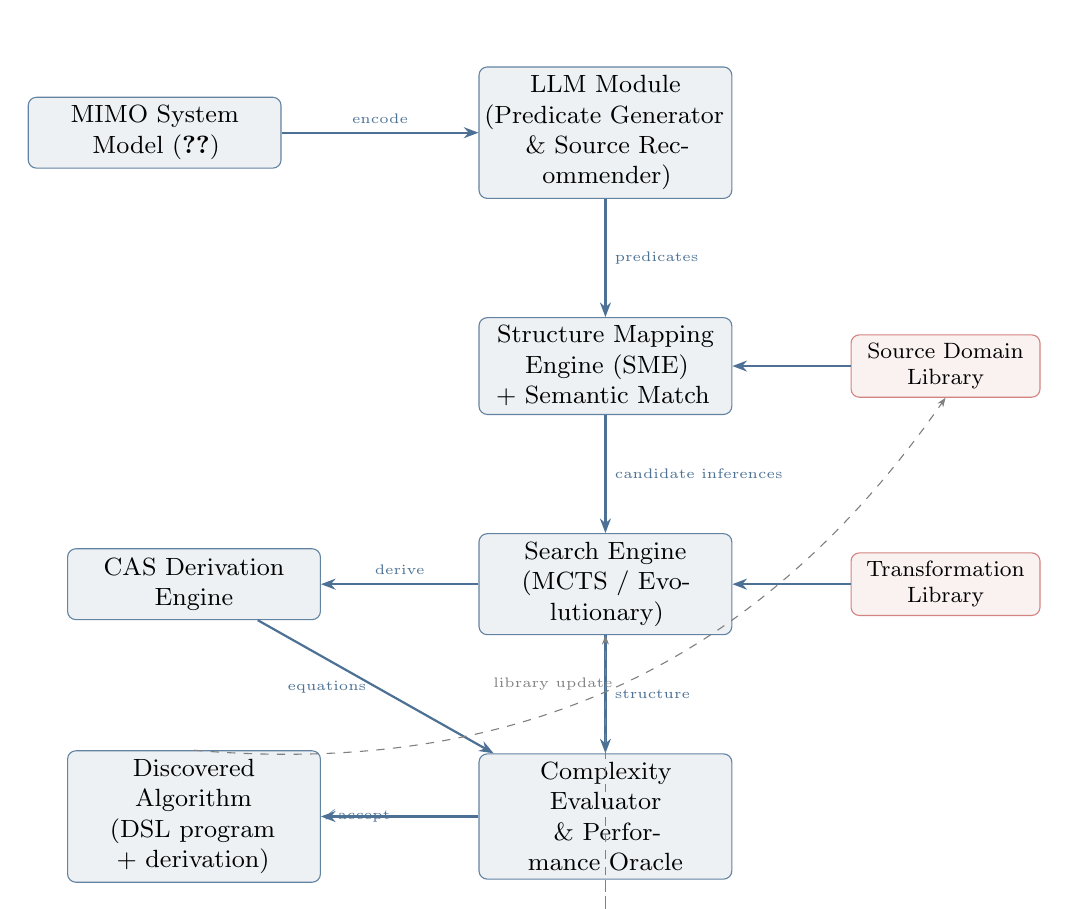
\begin{tikzpicture}[
  block/.style={draw=myblue!70, fill=myblue!8, rounded corners=3pt,
                minimum width=3.2cm, minimum height=0.9cm,
                font=\small, align=center, text width=3.0cm},
  smallblock/.style={draw=myorange!70, fill=myorange!8, rounded corners=3pt,
                minimum width=2.4cm, minimum height=0.7cm,
                font=\footnotesize, align=center},
  arrow/.style={-{Stealth[scale=0.8]}, thick, color=myblue!80},
  dasharrow/.style={-{Stealth[scale=0.7]}, dashed, color=gray},
  every node/.style={inner sep=3pt}
]

% Layer 1: Input
\node[block] (mimo) {MIMO System\\Model \eqref{eq:mimo}};

% Layer 2: LLM
\node[block, right=2.5cm of mimo] (llm) {LLM Module\\(Predicate Generator\\\& Source Recommender)};

% Layer 3: SME
\node[block, below=1.5cm of llm] (sme) {Structure Mapping\\Engine (SME)\\+ Semantic Match};

% Source domain DB
\node[smallblock, right=1.5cm of sme] (srcdb) {Source Domain\\Library};

% Layer 4: Search
\node[block, below=1.5cm of sme] (search) {Search Engine\\(MCTS / Evolutionary)};

% Layer 5: CAS
\node[block, left=2.0cm of search] (cas) {CAS Derivation\\Engine};

% Layer 6: Evaluator
\node[block, below=1.5cm of search] (eval) {Complexity Evaluator\\\& Performance Oracle};

% Output
\node[block, left=2.0cm of eval] (output) {Discovered\\Algorithm\\\small(DSL program + derivation)};

% Transformation lib
\node[smallblock, right=1.5cm of search] (translib) {Transformation\\Library};

% Arrows
\draw[arrow] (mimo) -- node[above,font=\tiny]{encode} (llm);
\draw[arrow] (llm) -- node[right,font=\tiny]{predicates} (sme);
\draw[arrow] (srcdb) -- (sme);
\draw[arrow] (sme) -- node[right,font=\tiny]{candidate inferences} (search);
\draw[arrow] (translib) -- (search);
\draw[arrow] (search) -- node[right,font=\tiny]{structure} (eval);
\draw[arrow] (search) -- node[above,font=\tiny]{derive} (cas);
\draw[arrow] (cas) -- node[left,font=\tiny]{equations} (eval);
\draw[arrow] (eval) -- node[left,font=\tiny]{\checkmark accept} (output);
\draw[dasharrow] (eval.south) -- ++(0,-0.5) -| (search.south);
\draw[dasharrow, bend right=30] (output.north) to node[left,font=\tiny]{library update} (srcdb.south);

\end{tikzpicture}
\caption{AlphaDetect system architecture.  Solid arrows denote primary data
flow; dashed arrows denote feedback (search pruning and library enrichment).}
\label{fig:architecture}
\end{figure}

The system operates as follows.  Given a MIMO system model, the LLM module
encodes it as a predicate structure and recommends candidate source domains.
The SME performs structural alignment between target and source domains,
producing candidate inferences that hypothesise new conceptual structures
(e.g., ``the MIMO system can be represented as a factor graph'').  The Search
Engine then navigates the space of DSL compositions and problem transformations,
guided by candidate inferences, type compatibility, and complexity constraints.
When a high-level algorithmic structure is selected, the CAS derives the exact
update equations.  The resulting algorithm is evaluated for complexity and
performance; successful discoveries are fed back to enrich the source-domain
library and DSL primitive set, enabling self-enlarging concept spaces.

% ══════════════════════════════════════════════════════════════════════════════
\section{Typed Domain-Specific Language}
\label{sec:dsl}
% ══════════════════════════════════════════════════════════════════════════════

\subsection{Design Philosophy}

The DSL serves as the \emph{semantic substrate} of AlphaDetect.  Every
expression in the DSL carries a precise type; every primitive comes with a
complexity annotation; every combinator is typed, so the type system
automatically enforces which combinations are legal without requiring
semantic understanding of the involved concepts.

\begin{tcolorbox}[insight]
  The type signature of a discovered intermediate object replaces human semantic
  understanding.  If the system constructs an object of type
  \texttt{FactorGraph[Variable, Factor]}, all algorithms that accept
  a \texttt{FactorGraph} as input become immediately applicable---regardless
  of whether the system ``understands'' what a factor graph means.
\end{tcolorbox}

\subsection{Type Hierarchy}

The DSL organises types in four layers.

\paragraph{Layer 0 --- Mathematical foundations.}
Scalars, tensors, matrices with structural subtypes
(Hermitian, PositiveDefinite, UpperTriangular, Unitary, etc.).

\paragraph{Layer 1 --- Signal-processing objects.}
\texttt{MIMOSystem}, \texttt{Constellation}, \texttt{SoftEstimate},
\texttt{HardEstimate}, \texttt{LLR}, \texttt{Subspace}.

\paragraph{Layer 2 --- Probabilistic / graph-model objects.}
\begin{itemize}[itemsep=0pt]
  \item \texttt{Distribution[X]} $\supset$ \texttt{Gaussian[X]},
        \texttt{DiscreteDistribution[X]}, \texttt{MixtureDist[X]}
  \item \texttt{Belief} $\supset$ \texttt{GaussianBelief},
        \texttt{DiscreteBelief}
  \item \texttt{BeliefSet[n]} $\supset$ \texttt{GaussianBeliefSet[n]},
        \texttt{DiscreteBeliefSet[n]}
  \item \texttt{Graph[Node,Edge]} $\supset$ \texttt{Tree},
        \texttt{BipartiteGraph} $\supset$ \texttt{FactorGraph},
        \texttt{WeightedGraph}
  \item \texttt{SearchTree[State]}, \texttt{CandidateList[T,Score]}
\end{itemize}

\paragraph{Layer 3 --- Algorithm-control objects.}
\texttt{Ordering}, \texttt{Heuristic}, \texttt{Criterion},
\texttt{Complexity}.

\subsection{Primitive Operations}

Selected primitives illustrating the DSL's scope are listed in
Table~\ref{tab:primitives}.

\begin{table}[H]
  \centering
  \caption{Representative DSL primitives with type signatures and complexity.}
  \label{tab:primitives}
  \small
  \begin{tabular}{@{}p{3.8cm}p{7.2cm}r@{}}
    \toprule
    \textbf{Primitive} & \textbf{Type Signature} & \textbf{Complexity} \\
    \midrule
    \texttt{qr} & $\mathtt{Matrix}[m,n]\to(\mathtt{Unitary}[m]\times\mathtt{UpperTriangular})$ & $O(mn^2)$ \\
    \texttt{mmse\_equalize} & $\mathtt{MIMOSystem}\to(\mathtt{SoftEstimate},\mathtt{ErrorCov})$ & $O(N_t^3)$ \\
    \texttt{system\_to\_factor\_graph} & $\mathtt{MIMOSystem}\to\mathtt{FactorGraph}$ & $O(N_rN_t)$ \\
    \texttt{find\_spanning\_tree} & $\mathtt{WeightedGraph}\to\mathtt{Tree}$ & $O(E\log V)$ \\
    \texttt{gaussian\_bp\_message} & $(\mathtt{Factor},\mathtt{GaussianMessages})\to\mathtt{GaussianMessage}$ & $O(N_t)$ \\
    \texttt{bp\_message\_factor\_to\_var} & $(\mathtt{Factor},\mathtt{Messages})\to\mathtt{Message}$ & $O(M^d)$ \\
    \texttt{sic\_detect\_one} & $(\mathtt{MIMOSystem},\mathtt{Int},\mathtt{Partial})\to(\mathtt{Symbol},\mathtt{MIMOSystem})$ & $O(N_rN_t)$ \\
    \texttt{expand\_node} & $(\mathtt{SearchTree},\mathtt{State})\to\mathtt{List[State,Cost]}$ & $O(M)$ \\
    \texttt{select\_top\_k} & $(\mathtt{CandidateList},k)\to\mathtt{CandidateList}$ & $O(n\log k)$ \\
    \texttt{mutual\_info\_weights} & $(\mathtt{GaussianBeliefSet},\mathtt{MIMOSystem})\to\mathtt{WeightedGraph}$ & $O(N_t^2)$ \\
    \bottomrule
  \end{tabular}
\end{table}

\subsection{Algorithmic Combinators}

Combinators are \emph{higher-order typed operators} that compose primitives
without violating type safety.

\vspace{0.3em}
\begin{lstlisting}[style=dsl, caption={Core combinator signatures}]
sequence  : (Op[A->B], Op[B->C]) -> Op[A->C]
guide     : (Op[A x Heuristic -> B], Op[A -> Heuristic]) -> Op[A->B]
nest      : (IterOp[A->B], Op[SubProblem->SubResult]) -> Op[A->B]
iterate   : (Op[S->S], init:S, convergence:S*S->Bool) -> S
fold_layers : (LayerOp, Ordering[Nt], MIMOSystem) -> HardEstimate
refine    : (Op[A->B], Op[B*A->B], n_steps:Int) -> Op[A->B]
parallel_merge : (Op[A->B1], Op[A->B2], Op[(B1,B2)->C]) -> Op[A->C]
\end{lstlisting}

\subsection{Type-Adapter Library}

Adapters bridge incompatible types and are the primary mechanism by which
\emph{cross-paradigm combinations} are discovered.

\vspace{0.3em}
\begin{lstlisting}[style=dsl, caption={Key adapters bridging probabilistic beliefs and search control}]
beliefs_to_ordering    : BeliefSet[n] -> Ordering[n]
beliefs_to_heuristic   : BeliefSet[n] -> Heuristic[PartialSymbolVec -> Score]
beliefs_to_candidates  : DiscreteBeliefSet[n] -> CandidateList[SymbolVec, Prob]
estimate_to_beliefs    : (SoftEstimate[n], ErrorCov) -> GaussianBeliefSet[n]
covariance_to_graph    : PositiveDefinite[n] -> WeightedGraph[n, Real]
partial_to_reduced_sys : (MIMOSystem, PartialDecision[k]) -> MIMOSystem[Nt-k, Nr]
\end{lstlisting}

\noindent
The discovery of a new cross-paradigm algorithm reduces to finding a
type-correct path through primitives, combinators, and adapters.  The
search engine enumerates candidate paths; the complexity evaluator prunes
infeasible ones; performance on a benchmark channel model selects among
survivors.

% ══════════════════════════════════════════════════════════════════════════════
\section{Problem Transformation Library}
\label{sec:transform}
% ══════════════════════════════════════════════════════════════════════════════

\subsection{Transformations as Concept Generators}

The invention of an intermediate concept reduces to the \emph{application of a
problem transformation} whose output (the ``witness'') becomes the new object.
The transformation library catalogues known patterns, organised by category.

\begin{table}[H]
  \centering
  \caption{Problem transformation categories with typed signatures and witness objects.}
  \label{tab:transforms}
  \small
  \begin{tabular}{@{}p{2.6cm}p{7.8cm}p{2.6cm}@{}}
    \toprule
    \textbf{Category} & \textbf{Transformation} & \textbf{Witness} \\
    \midrule
    \textit{Algebraic} &
      $\mathtt{qr}$: $\bH \to \mathbf{Q}\mathbf{R}$ & $\mathbf{Q},\mathbf{R}$ \\
    &  $\mathtt{woodbury}$: $(A+UCV)^{-1}\to$ small inverse & interm.\ matrices \\
    &  $\mathtt{complete\_square}$: $f(x)\to g(x-h)^2+k$ & $h,k$ \\
    \midrule
    \textit{Probabilistic} &
      $\mathtt{introduce\_latent}$: $p(\bx)\to\int p(\bx,\mathbf{z})\,d\mathbf{z}$ & $\mathbf{z}$ \\
    &  $\mathtt{factorize\_joint}$: $p(\bx_{1:n})\to\prod p(x_i|pa_i)$ & graph, CPDs \\
    &  $\mathtt{exponential\_family}$: $p\to\exp(\theta^\top T(x)-A(\theta))$ & $\theta$, $T$ \\
    \midrule
    \textit{Optimisation} &
      $\mathtt{lagrangian\_relax}$: $\min f\;\mathrm{s.t.}\; g\le 0 \to \min_x\max_\lambda\mathcal{L}$ & $\lambda$ \\
    &  $\mathtt{coordinate\_descent}$: $\min_{x,y}f\to$ alternating mins & sub-objectives \\
    &  $\mathtt{surrogate\_objective}$: $f\to\tilde{f}\ge f$ & surrogate, bound \\
    \midrule
    \textit{Structural} &
      $\mathtt{to\_factor\_graph}$: system $\to$ \texttt{FactorGraph} & factor nodes \\
    &  $\mathtt{tree\_approximate}$: \texttt{Graph} $\to$ \texttt{Tree} & tree, approx err.\ \\
    \bottomrule
  \end{tabular}
\end{table}

\subsection{Searchability of the Transformation Space}

Applying a transformation $T$ to the current problem yields a witness and a
transformed sub-problem.  The sub-problem is matched against known solvable
patterns (within the DSL type system).  Two signals indicate a useful
transformation:
\begin{itemize}[itemsep=0pt]
  \item The transformed problem has a \emph{lower complexity class}; or
  \item The transformed problem \emph{type-matches} the input of a known
        efficient algorithm.
\end{itemize}

\noindent
The search engine navigates the transformation space using a
complexity-guided heuristic: transformations that reduce complexity class
or increase structural constraint are preferred.

% ══════════════════════════════════════════════════════════════════════════════
\section{CAS-Driven Derivation Engine}
\label{sec:cas}
% ══════════════════════════════════════════════════════════════════════════════

\subsection{Role of the CAS}

Once the search engine has selected a high-level algorithmic structure
(which primitives, which combinators, which transformation sequence), the
CAS takes over to derive the exact update equations.  The CAS does not
invent concepts; it performs:
\begin{enumerate}[itemsep=0pt]
  \item Symbolic expansion of objective functions (KL divergence, MSE, etc.)
  \item Functional differentiation and stationarity conditions
  \item Gaussian closure: marginalisation, conditioning, moment computation
  \item Complexity class determination via symbolic asymptotic analysis
\end{enumerate}

\subsection{CAS Implementation Details}

The CAS operates on symbolic expressions conforming to the DSL type system.
Key capabilities include:
\begin{itemize}[itemsep=0pt]
  \item \textbf{Gaussian algebra}: Given a joint Gaussian
        $\calN(\bmu,\bSigma)$, compute marginals, conditionals, and Schur
        complements in closed form.
  \item \textbf{Exponential-family calculus}: Given a distribution in
        exponential-family form $\exp(\theta^\top T(x)-A(\theta))$, compute
        natural gradients, sufficient statistics, and moment parameters.
  \item \textbf{KL divergence expansion}: Symbolically expand
        $\KL(q\|p)$ or $\KL(p\|q)$ for parametric families and derive
        stationarity conditions with respect to variational parameters.
  \item \textbf{Precision-domain arithmetic}: Maintain beliefs in precision
        (information) form to enable efficient cavity computations via
        subtraction rather than matrix inversion.
  \item \textbf{Asymptotic complexity analysis}: Given a symbolic expression,
        determine the asymptotic complexity class in $N_t$, $N_r$, and $M$.
\end{itemize}

% ══════════════════════════════════════════════════════════════════════════════
\section{LLM-Augmented Structure Mapping Engine}
\label{sec:sme}
% ══════════════════════════════════════════════════════════════════════════════

\subsection{Structure Mapping Theory}

Gentner's Structure Mapping Theory (SMT) \cite{gentner1983} posits that
analogy is not surface similarity but \emph{structural alignment}: a bijective
mapping between the relational structures of a source domain and a target
domain.  The three guiding principles are:

\begin{enumerate}[leftmargin=2em, itemsep=2pt]
  \item \textbf{Structural consistency}: the mapping is one-to-one.
  \item \textbf{Systematicity principle}: higher-order relational structure
        (relations-among-relations) is preferred over isolated attribute matches.
  \item \textbf{Candidate inferences}: predicates that exist in the source
        but have no target counterpart are \emph{predicted} to potentially
        hold in the target---this is the mechanism for knowledge transfer.
\end{enumerate}

\noindent
The Structure Mapping Engine (SME) \cite{falkenhainer1989} implements SMT
computationally, producing \emph{gmaps} (globally consistent mappings) ranked
by structural evaluation score.

\subsection{The Representation Bottleneck and LLM Resolution}

SME requires domains to be described as hand-crafted predicate structures.
Chalmers et al.\ \cite{chalmers1992} criticised this: the creative work may
reside in the representation design rather than in SME itself.
AlphaDetect resolves this by using an LLM as an automated predicate generator.

A fine-tuned (or few-shot prompted) LLM encodes mathematical
concepts as predicate structures conforming to the DSL's ontology:

\vspace{0.3em}
\begin{lstlisting}[style=dsl, caption={LLM-generated predicate encoding of the MIMO posterior inference problem}]
;; Target domain: MIMO posterior inference
(coupled-variables x1 ... xNt H)
(intractable exact-marginal posterior)
(goal marginal-inference posterior x_i)
(additive-noise observation sigma-squared)
(constraint discrete-valued x constellation)
(complexity-target polynomial)
\end{lstlisting}

\begin{lstlisting}[style=dsl, caption={LLM-generated predicate encoding of factor-graph inference (source domain)}]
;; Source domain: Factor-graph probabilistic inference
(coupled-variables v1 ... vN factor-graph)
(factorized-distribution p factors)
(graph-structure factor-graph variables factors)
(message-passing bp factor-graph)
(tractable message-passing tree)
(intractable exact-message-passing general-graph)
(tree-decomposition general-graph tree)
(optimality Chow-Liu KL-optimal-tree-approximation)
\end{lstlisting}

\subsection{SME Matching and Candidate Inferences}

Running SME on the two predicate sets produces the following global mapping:

\vspace{0.3em}
\noindent
\begin{tabular}{@{}ll@{}}
  \toprule
  \textbf{Source (factor-graph inference)} & \textbf{Target (MIMO detection)} \\
  \midrule
  \texttt{coupled-variables vi (factor-graph)} & \texttt{coupled-variables xi (H)} \\
  \texttt{intractable exact-message-passing} & \texttt{intractable exact-marginal} \\
  \texttt{goal marginal-inference} & \texttt{goal marginal-inference} \\
  \bottomrule
\end{tabular}

\vspace{0.6em}
\noindent
\textbf{Candidate inferences} (source predicates absent from target):
\begin{enumerate}[itemsep=2pt]
  \item \texttt{(graph-structure ??? variables factors)}
        $\Rightarrow$ \emph{MIMO system can be represented as a factor graph.}
  \item \texttt{(message-passing bp ??? $\to$ marginals)}
        $\Rightarrow$ \emph{BP can be applied to the MIMO factor graph.}
  \item \texttt{(tree-decomposition ??? tree)}
        $\Rightarrow$ \emph{Approximate MIMO factor graph with a spanning tree.}
\end{enumerate}

These three inferences, in sequence, correspond precisely to the conceptual
steps that led human researchers to GTA.

\subsection{LLM-Augmented Semantic Matching}

Standard SME requires identical predicate names (functors) to produce a match.
We replace this with LLM-embedding cosine similarity:

\begin{equation}
  m(\pi_s, \pi_t) = \frac{\mathbf{e}_s^\top \mathbf{e}_t}{\|\mathbf{e}_s\|\|\mathbf{e}_t\|},
  \qquad \mathbf{e} = \mathrm{LLM\_embed}(\text{functor} \oplus \text{args description})
\end{equation}

This allows SME to discover analogies across vocabularies (e.g.\
\texttt{propagate} $\leftrightarrow$ \texttt{transmit}) and across domains
encoded by different research communities.

\subsection{LLM as Source-Domain Recommender}

Given the target predicate set, the LLM recommends candidate source domains by
ranking mathematical/engineering areas by estimated structural similarity.  For
MIMO detection, typical recommendations include: statistical physics (Ising
inference), LDPC decoding, Markov random field labelling, lattice reduction,
and convex optimisation.  Each recommended domain is then encoded into
predicates by the LLM, and SME computes formal Gmap scores.

% ══════════════════════════════════════════════════════════════════════════════
\section{Search Engine and Evaluation}
\label{sec:search}
% ══════════════════════════════════════════════════════════════════════════════

\subsection{Search Strategy}

The Search Engine navigates the combined space of DSL compositions, problem
transformations, and SME-suggested conceptual hypotheses.  It employs two
complementary strategies:

\begin{itemize}[itemsep=2pt]
  \item \textbf{MCTS (Monte Carlo Tree Search)}: Each node in the search tree
        represents a partial algorithm (a sequence of DSL operations and
        transformations applied so far).  Expansion adds one more primitive,
        combinator, or transformation.  Rollout estimates performance via
        lightweight simulation on small MIMO instances.  The UCB1 criterion
        balances exploration and exploitation.
  \item \textbf{Evolutionary search}: A population of candidate DSL programs
        evolves via mutation (replace one primitive), crossover (swap
        sub-expressions between two programs), and selection (retain programs
        with best performance-to-complexity ratio).
\end{itemize}

\subsection{Complexity Evaluator}

Every candidate algorithm is annotated with a symbolic complexity expression
derived from the CAS.  The evaluator gates the search by rejecting candidates
whose complexity exceeds a user-specified budget (e.g., $O(N_t^3)$ for
real-time detection).

\subsection{Performance Oracle}

Candidate algorithms that pass the complexity gate are evaluated on a benchmark
suite comprising:
\begin{itemize}[itemsep=0pt]
  \item Rayleigh i.i.d.\ channels ($N_t = N_r = 16, 32, 64$)
  \item Correlated channels (exponential correlation model)
  \item Ill-conditioned channels (condition number $> 100$)
  \item Multiple constellations (QPSK, 16-QAM, 64-QAM)
\end{itemize}
Performance is measured by BER at target SNR values.  Algorithms that achieve
BER improvements over the best known baseline for any scenario are flagged
for human review.

\subsection{Concept Space Self-Enlargement}

A key design feature is the \emph{self-enlarging concept space}:
\begin{enumerate}[itemsep=0pt]
  \item Successful algorithm compositions are added to the source-domain
        library (SME) and as new primitives (DSL) via Library
        Learning \cite{dreamcoder2021}.
  \item The enriched libraries enable higher-order conceptual transfer that
        was impossible with the initial primitive set.
\end{enumerate}
This mirrors the DreamCoder wake--abstraction--dream cycle, applied to
algorithm discovery rather than program synthesis.

% ══════════════════════════════════════════════════════════════════════════════
\section{Case Studies}
\label{sec:cases}
% ══════════════════════════════════════════════════════════════════════════════

We now demonstrate, through three detailed case studies, how known MIMO
detection algorithms can be re-derived within the AlphaDetect framework.  Each
case study traces the full path from problem specification to final algorithm,
showing which components of the system are invoked at each step.

\subsection{Case Study 1: Automatic Derivation of EP-MIMO}
\label{sec:ep_derivation}

Expectation Propagation (EP) for MIMO detection \cite{minka2001} is an
algorithm whose core innovations---the cavity distribution, the tilted
distribution, and moment matching---are often presented as creative insights.
We show that all these ``concepts'' emerge as algebraic by-products of the
CAS derivation engine, given appropriate search decisions.

\paragraph{Setup.}
The Bayesian posterior is
\begin{equation}
  p(\bx|\by) \propto \underbrace{\calN(\by;\bH\bx,\sigma^2\bI)}_{f_0(\bx)}
  \cdot \prod_{i=1}^{N_t}\underbrace{p(x_i)}_{f_i(x_i)}.
  \label{eq:posterior}
\end{equation}
Exact marginalisation is $O(M^{N_t})$, flagged as infeasible by the complexity
evaluator.

\paragraph{Search decision 1 --- Approximate in Gaussian family.}
The search engine selects
$\mathtt{approximate\_in\_family}(p,\;\mathtt{Gaussian},\;\KL_\text{reverse})$,
producing witness $q(\bx)=\calN(\bmu,\bSigma)$.

\paragraph{Search decision 2 --- Match factorisation.}
The search engine applies $\mathtt{match\_factorization}$, yielding
$q(\bx)\propto f_0(\bx)\cdot\prod_i \tilde{q}_i(x_i)$
with site approximations $\tilde{q}_i=\calN(\mu_i,\sigma_i^2)$ as witnesses.

\paragraph{Search decision 3 --- Coordinate descent.}
The search engine selects $\mathtt{coordinate\_descent}$ over the $\tilde{q}_i$.
The CAS then derives the optimal update for $\tilde{q}_i$
with all other factors fixed:

\begin{align}
  \underbrace{q_{-i}(\bx) \triangleq \frac{q(\bx)}{\tilde{q}_i(x_i)}}_{\text{\emph{cavity distribution (CAS witness)}}}
  &= \calN(\bmu_{-i},\bSigma_{-i})
  \label{eq:cavity}\\[4pt]
  \underbrace{\hat{p}_i(x_i) \propto f_i(x_i)\cdot q_{-i}^{\mathrm{marg}}(x_i)}_{\text{\emph{tilted distribution (CAS witness)}}}
  &= \sum_{s\in\calS} w_s\,\delta(x_i-s),\quad
  w_s \propto \calN(s;\mu_{-i},\sigma_{-i}^2)
  \label{eq:tilted}\\[4pt]
  \tilde{q}_i^\mathrm{new}:\quad
  &\Exp_{\hat{p}_i}[x_i],\;\Var_{\hat{p}_i}[x_i]
  \quad\leftarrow\quad O(M)\text{ computation}
  \label{eq:moments}
\end{align}

The cavity parameters are obtained by precision-domain subtraction (CAS step):
\begin{equation}
  \sigma_{-i}^{-2} = \sigma_{q,i}^{-2} - \sigma_{\tilde{q}_i}^{-2},\qquad
  \mu_{-i}\sigma_{-i}^{-2} = \mu_{q,i}\sigma_{q,i}^{-2} - \mu_{\tilde{q}_i}\sigma_{\tilde{q}_i}^{-2}.
  \label{eq:precision}
\end{equation}

\begin{tcolorbox}[insight]
  From the CAS perspective, \emph{cavity distribution} and
  \emph{tilted distribution} are merely intermediate algebraic quantities
  introduced to simplify expressions.  Human researchers gave them names and
  intuitions; the CAS required neither.
\end{tcolorbox}

\paragraph{Complexity verification.}
The full EP iteration has complexity $O(N_\text{iter}\cdot N_t\cdot(N_t^2+M))$,
which is polynomial---accepted by the evaluator.

\paragraph{Multi-path exploration.}
Different search decisions yield different algorithms:

\vspace{0.3em}
\begin{tabular}{llll}
  \toprule
  \textbf{KL direction} & \textbf{Factorisation} & \textbf{Family} & \textbf{Algorithm} \\
  \midrule
  $\KL(q\|p)$ & Match prior & Gaussian & \textbf{EP-MIMO} \\
  $\KL(q\|p)$ & Mean field & Exponential family & Variational Bayes \\
  $\KL(p\|q)$ & Match prior & Gaussian & $\alpha$-divergence approx. \\
  -- & -- & Gaussian + Laplace & Laplace-EP \\
  \bottomrule
\end{tabular}

\paragraph{DSL representation of EP-MIMO.}
\begin{align}
  &\texttt{sites}_0 = \texttt{init\_gaussian\_sites}(N_t) \notag\\
  &\hat{\bx} = \texttt{iterate}\bigl(\texttt{ep\_update\_step}(\textit{sys}, \texttt{sites}),\;
               \texttt{sites}_0,\; \text{convergence}\bigr) \notag
\end{align}
where \texttt{ep\_update\_step} internally invokes the CAS-derived cavity
computation, tilted distribution formation, and moment matching.

\subsection{Case Study 2: Gaussian Tree Approximation (GTA)}
\label{sec:gta}

GTA \cite{gta2006} exemplifies a \emph{structural innovation}: the key insight
is to approximate the fully-connected MIMO factor graph with an optimal spanning
tree.  This case study demonstrates how the SME module drives discovery of
structural concepts that the CAS alone cannot derive.

\paragraph{SME-driven hypothesis generation.}
Given the MIMO posterior inference problem as the target domain, the LLM
recommends factor-graph inference as a candidate source domain.  SME alignment
produces the candidate inference: ``the MIMO system can be represented as a
factor graph, and the factor graph can be approximated by a spanning tree.''

\paragraph{DSL program.}
The search engine, guided by the SME candidate inference, constructs:
\begin{align}
  &\texttt{beliefs}_0 = \texttt{estimate\_to\_beliefs}(\texttt{mmse\_equalize}(\textit{sys})) \notag\\
  &\texttt{weights} = \texttt{mutual\_info\_weights}(\texttt{beliefs}_0,\; \textit{sys}) \notag\\
  &\texttt{tree} = \texttt{find\_spanning\_tree}(\texttt{weights},\; \textit{objective}=\max) \notag\\
  &\hat{\bx} = \texttt{iterate}(\texttt{gaussian\_bp\_on\_tree}(\texttt{tree}),\;\texttt{beliefs}_0,\;\text{convergence}) \notag
\end{align}

\paragraph{CAS role.}
The CAS derives the Gaussian BP message equations on the tree structure.  Its
role is secondary: solving the message-passing update equations once the tree
structure is given.

\paragraph{Key discovery bottleneck.}
The Chow-Liu weight function (mutual information between variable pairs) is the
critical choice that cannot be derived from an objective function alone.  It
requires either (a)~the SME to transfer the Chow-Liu optimality result from
information theory, or (b)~the search engine to evaluate multiple candidate
weight functions on the benchmark.

\subsection{Case Study 3: BP-Guided Sphere Decoding}
\label{sec:bpsd}

BP-guided sphere decoding exemplifies \emph{algorithmic combination}: two
existing paradigms (belief propagation and tree search) are composed via
type adapters to produce a superior hybrid.

\paragraph{DSL program.}
\begin{align}
  &\texttt{beliefs} = \texttt{iterate}(\texttt{gaussian\_bp\_message},\; \texttt{fg},\; 5\text{ steps}) \notag\\
  &\texttt{ordering} = \texttt{beliefs\_to\_ordering}(\texttt{beliefs}) \notag\\
  &\hat{\bx} = \texttt{best\_first\_search}(\texttt{tree}(\textit{sys},\texttt{ordering}),\;
                \texttt{beliefs\_to\_heuristic}(\texttt{beliefs}),\; K) \notag
\end{align}

\paragraph{Discovery mechanism.}
The search engine finds this combination by enumerating type-correct paths:
\texttt{gaussian\_bp\_message} produces a \texttt{GaussianBeliefSet};
the adapter \texttt{beliefs\_to\_ordering} converts it to an \texttt{Ordering}
required by tree search; the adapter \texttt{beliefs\_to\_heuristic} converts
it to a \texttt{Heuristic} for pruning.  No structural analogy or CAS
derivation is needed---pure type-guided composition suffices.

\paragraph{DSL representation of OSIC.}
As a further combination example, BLAST with MMSE ordering (OSIC) is:
\begin{equation}
  \hat{\bx} = \texttt{fold\_layers}\bigl(\texttt{sic\_detect\_one},\;
              \texttt{beliefs\_to\_ordering}(\texttt{estimate\_to\_beliefs}(\cdot)),\;
              \textit{sys}\bigr) \notag
\end{equation}

\subsection{Discoverability Comparison}

\begin{table}[H]
  \centering
  \caption{Automated discoverability comparison across the three case studies.}
  \label{tab:discoverability}
  \small
  \begin{tabular}{@{}p{3.0cm}p{3.0cm}p{3.0cm}p{3.5cm}@{}}
    \toprule
    \textbf{Aspect} & \textbf{EP-MIMO} & \textbf{GTA} & \textbf{BP-Guided SD} \\
    \midrule
    Innovation type & Optimisation & Structural & Combination \\
    Primary component & CAS & SME + Search & DSL type search \\
    Key conceptual leap & CAS-derivable & Tree approx.\ (structural) & Type adapter \\
    CAS role & Central & Minor & None \\
    SME role & None & Central & None \\
    Difficulty & Medium & Medium--High & Low--Medium \\
    Bottleneck & KL dir.\ + factorisation & Chow-Liu weight fn.\ & None significant \\
    \bottomrule
  \end{tabular}
\end{table}

\noindent
\textbf{Key finding.}  EP is more derivable under the CAS because its core
innovations arise from optimisation decomposition---a purely algebraic
process---whereas GTA's tree approximation is a structural selection requiring
cross-domain analogical reasoning.  BP-guided sphere decoding is the most
easily discoverable, requiring only type-guided composition.

% ══════════════════════════════════════════════════════════════════════════════
\section{Discussion: Scope and Limitations}
\label{sec:discussion}
% ══════════════════════════════════════════════════════════════════════════════

\subsection{DSL Granularity Trade-off}

The most critical design choice in AlphaDetect is the granularity of the DSL:

\begin{itemize}[itemsep=2pt]
  \item \textbf{Too coarse} (only matrix operations): GTA and EP cannot be
        derived because the factor-graph type does not exist.
  \item \textbf{Too fine} (tree approximation as a primitive): the discovery
        is trivially guided; the system has been told the answer.
  \item \textbf{Target granularity}: Include the individual components of the
        solution (factor graph type, spanning tree algorithm, message passing
        step, moment computation) but not pre-assembled combinations.
        The ``weight function for Chow-Liu'' is discovered, not given.
\end{itemize}

\subsection{The Irreducible Role of Structural Intuition}

The GTA analysis reveals a fundamental asymmetry:
\emph{optimisation-based} innovations (EP, EM, ADMM) are CAS-derivable once
the objective and factorisation are chosen, while \emph{structure-based}
innovations (tree approximation, lattice representation of MIMO) require
cross-domain analogical reasoning.  No formal mechanism fully automates
structural intuition; SME provides a systematic---but imperfect---surrogate.

\subsection{Axiomatic Probing as a Semantic Fallback}

When a discovered intermediate object has no type in the DSL (e.g., because it
emerged from a neural component), \emph{axiomatic probing} provides a semantic
fallback:
\begin{itemize}[itemsep=0pt]
  \item Test whether the object satisfies graph axioms (adjacency, no-cycle) $\Rightarrow$ assign \texttt{Tree} type.
  \item Test metric axioms (non-negativity, symmetry, triangle inequality) $\Rightarrow$ \texttt{Metric} type.
  \item Test Gaussian moment conditions $\Rightarrow$ \texttt{GaussianDistribution} type.
\end{itemize}
Once typed, the object can participate in typed DSL compositions.

% ══════════════════════════════════════════════════════════════════════════════
\section{Related Work}
\label{sec:related}
% ══════════════════════════════════════════════════════════════════════════════

\begin{description}[leftmargin=0em, labelwidth=0em, itemsep=4pt]
  \item[Gentner (1983) \cite{gentner1983}]
    Structure Mapping Theory: analogy as relational structure alignment.
    Foundation for AlphaDetect's cross-domain transfer mechanism.

  \item[Falkenhainer, Forbus \& Gentner (1989) \cite{falkenhainer1989}]
    Structure Mapping Engine: the algorithmic implementation of SMT.
    AlphaDetect extends SME with LLM-based semantic matching.

  \item[Ellis et al.\ (2021) \cite{dreamcoder2021}]
    DreamCoder: library learning by abstracting shared program fragments.
    AlphaDetect adopts the wake--abstraction--dream cycle for the
    concept self-enlargement mechanism.

  \item[Chalmers, French \& Hofstadter (1992) \cite{chalmers1992}]
    Critique of AI methodology regarding the representation bottleneck in
    analogy.  Directly motivates our LLM-based predicate generation.

  \item[Minka (2001) \cite{minka2001}]
    Expectation Propagation for approximate Bayesian inference.
    The algorithm re-derived in Case Study 1.

  \item[Turney (2008) \cite{turney2008}]
    Latent Relation Mapping Engine: SME without hand-coded LISP input,
    using vector-space representations.  Directly relevant to our
    LLM-embedding extension of SME matching.
\end{description}

% ══════════════════════════════════════════════════════════════════════════════
\section{Summary and Contributions}
\label{sec:summary}
% ══════════════════════════════════════════════════════════════════════════════

AlphaDetect addresses the hard problem of \emph{explainable algorithm discovery}
for MIMO detection.  Its principal contributions are:

\begin{enumerate}[leftmargin=2em, itemsep=4pt]
  \item \textbf{Formal characterisation of conceptual innovation.}  We identify
        three forms (structural analogy, optimisation-driven derivation,
        algorithmic combination) and map each to a tractable automated mechanism.

  \item \textbf{Typed DSL with algorithmic combinators and adapters.}  The DSL
        provides a type-safe compositional language in which known algorithms
        can be expressed and new ones searched.

  \item \textbf{Problem transformation library.}  Intermediate variable
        invention is recast as witness generation from typed transformations,
        converting an open-ended creative act into structured search.

  \item \textbf{CAS integration for automatic algorithm derivation.}  We show
        that EP-MIMO and all its variants can be derived by CAS-driven
        coordinate descent, with cavity and tilted distributions emerging as
        algebraic by-products.

  \item \textbf{LLM-augmented Structure Mapping Engine.}  LLMs are used as
        predicate generators and source-domain recommenders---providing semantic
        bridging---while SME enforces formal structural consistency and
        generates candidate inferences that drive the search.

  \item \textbf{Unified system architecture.}  The four components
        (DSL, transformations, CAS, SME) are integrated into a coherent
        system with MCTS/evolutionary search, complexity evaluation,
        performance benchmarking, and self-enlarging concept spaces.

  \item \textbf{Comprehensive case studies.}  We demonstrate through EP-MIMO,
        GTA, and BP-guided sphere decoding that the framework covers all three
        innovation types, from pure algebraic derivation to cross-domain
        structural analogy to type-guided algorithmic combination.
\end{enumerate}

% ══════════════════════════════════════════════════════════════════════════════
\begin{thebibliography}{9}

\bibitem{gentner1983}
D.~Gentner,
``Structure-mapping: A theoretical framework for analogy,''
\textit{Cognitive Science}, vol.~7, no.~2, pp.~155--170, 1983.

\bibitem{falkenhainer1989}
B.~Falkenhainer, K.~D.~Forbus, and D.~Gentner,
``The structure-mapping engine: Algorithm and examples,''
\textit{Artificial Intelligence}, vol.~41, no.~1, pp.~1--63, 1989.

\bibitem{dreamcoder2021}
K.~Ellis, C.~Wong, M.~Nye, M.~Sable-Meyer, L.~Cary, L.~Morales, L.~Hewitt,
A.~Solar-Lezama, and J.~Tenenbaum,
``DreamCoder: Bootstrapping inductive program synthesis with wake-sleep library learning,''
\textit{Proc.\ ACM PLDI}, 2021.

\bibitem{turney2008}
P.~D.~Turney,
``The latent relation mapping engine: Algorithm and experiments,''
\textit{Journal of Artificial Intelligence Research}, vol.~33, pp.~615--655, 2008.

\bibitem{chalmers1992}
D.~J.~Chalmers, R.~M.~French, and D.~R.~Hofstadter,
``High-level perception, representation, and analogy: A critique of artificial intelligence methodology,''
\textit{Journal of Experimental \& Theoretical Artificial Intelligence},
vol.~4, no.~3, pp.~185--211, 1992.

\bibitem{minka2001}
T.~P.~Minka,
``Expectation propagation for approximate Bayesian inference,''
\textit{Proc.\ UAI}, pp.~362--369, 2001.

\bibitem{gta2006}
C.~Choi and A.~Singer,
``A tree-reweighted belief propagation algorithm for restoring sparse signals,''
\textit{Proc.\ ICASSP}, 2006.

\bibitem{colton2002}
S.~Colton,
\textit{Automated Theory Formation in Pure Mathematics}.
Springer, 2002.

\end{thebibliography}

\end{document}
